\documentclass[journal]{IEEEtran}
\usepackage{amsmath,amssymb,amsfonts,amsthm}
\usepackage{graphicx}
\usepackage{booktabs}
\usepackage{multirow}
\usepackage{algorithm}
\usepackage[noend]{algpseudocode}
\usepackage[caption=false,font=footnotesize]{subfig}
\usepackage{xcolor}
\usepackage[colorlinks=true,linkcolor=blue,citecolor=blue,urlcolor=blue]{hyperref}
\usepackage{balance}

\newtheorem{proposition}{Proposition}
\newtheorem{assumption}{Assumption}
\newtheorem{remark}{Remark}

\graphicspath{{figs/}}

\newcommand{\ehat}{\hat{c}}
\newcommand{\E}{\mathbb{E}}
\newcommand{\R}{\mathbb{R}}

% --- numbers filled from results/boundary and results/recoverability ---
\newcommand{\boundaryreactive}{the three trained policies fall from about
ninety percent at nominal to a $0.08$--$0.23$ band at full severity, no better
than a blind walk}
\newcommand{\boundaryoracle}{$0.70$--$0.90$ --- the encoder fault is nearly a
non-event when the bearing is trustworthy}
\newcommand{\recovnumbers}{A \emph{linear} read-out of either representation is
useless (rotation $R^2 \approx 0.00$); a non-linear decoder recovers the true
turn rate only weakly (raw depth $R^2 \approx 0.60$, the VAE latent flow
$R^2 \approx 0.49$) and forward speed not at all ($R^2 < 0$ for both, a
forward depth profile scarcely changing as the robot advances).}

\begin{document}

\title{PROTEUS: When Does Identifying the Body Help?\\
Embodiment-Context Adaptation and Its Limits for\\
Actuation-Fault-Robust Visual Navigation}

\author{Tuan~Anh~Nguyen,
        Uiseok~Lee,
        Eunmi~Choi,
        and~Dugki~Min%
\thanks{T. A. Nguyen is with the Faculty of Information Technology, HUIT,
Ho Chi Minh City, Vietnam (e-mail: anhngt@huit.edu.vn).}%
\thanks{U. Lee and D. Min are with the Department of Computer Science and
Engineering, Konkuk University, Seoul, South Korea.}%
\thanks{E. Choi is with the School of Software, Kookmin University, Seoul,
South Korea.}}

\markboth{IEEE Transactions (under review)}{Nguyen \MakeLowercase{\textit{et
al.}}: PROTEUS: Privileged Embodiment-Context Distillation}

\maketitle

\begin{abstract}
% ~200 words, no numerals
Vision-based deep reinforcement learning yields capable mapless navigation
policies, and a growing literature hardens them against degraded perception
and moving obstacles. A complementary vulnerability is the robot's own
actuation: motor wear, trim drift, control latency, traction slip, and speed
droop reshape how commands become motion, so a policy tuned to one body may
veer or stall while its perception stays flawless. Borrowing the
privileged-distillation philosophy that transformed legged locomotion, we
develop PROTEUS, a complete framework that treats the embodiment as a latent
context identified online: a privileged teacher trained on the true fault
parameters under a self-paced severity curriculum, distilled into a deployable
student that infers the context from command--response history fused with
visual latent flow. We release FaultNav, a reproducible simulator whose
wheel-space fault operator injects faults where physical faults act. Building
the system in full, however, let us ask a sharper question than whether it
works: when should it help at all? Through controlled experiments we establish
a boundary. Under reliable localization the studied actuation faults prove
largely feedback-compensable, so identification earns little; the single
regime where embodiment knowledge would pay --- corrupted proprioception ---
demands an exteroceptive motion reference that a forward depth sensor cannot
supply. We characterize this compensability-and-observability boundary
analytically and empirically, delineating where embodiment adaptation is worth
its cost and where reactive feedback already suffices.
\end{abstract}

\begin{IEEEkeywords}
Autonomous navigation, deep reinforcement learning, actuation faults,
embodiment adaptation, privileged distillation, variational autoencoder,
fault tolerance, mobile robots.
\end{IEEEkeywords}

\IEEEpeerreviewmaketitle

\section{Introduction}
\IEEEPARstart{L}{earned} visual navigation has matured from a laboratory
curiosity into a practical control paradigm: an encoder compresses raw
exteroception into a compact latent state, and an actor--critic learner maps
that latent, together with goal information, into continuous velocity
commands~\cite{Tai2017VirtualToReal,Zhu2021DRLNavSurvey}. Within this
paradigm, a line of work initiated by an attention-enhanced variational
autoencoder (VAE) coupled to a deterministic policy-gradient controller
demonstrated that carefully engineered \emph{perception} robustness ---
channel--spatial attention, multi-scale feature fusion, and
reconstruction-to-clean training --- lets a differential-drive robot navigate
reliably in illumination regimes where a plain end-to-end network
fails~\cite{Lee2026VAEDDPG}. Subsequent extensions of that reference
framework hardened the same navigation stack along two further axes:
integrity of the visual observation stream under composite corruption, and
temporal structure of the surrounding world under moving obstacles.

These advances share an assumption so ingrained that it is rarely stated:
the \emph{actuation channel is intact}. Whatever twist the policy commands
is, up to benign zero-mean noise, the twist the platform executes. Field
experience contradicts this premise constantly. Motor drivers lose gain as
temperature rises; differential platforms develop per-wheel asymmetries from
unequal wear or tire pressure; miscalibrated trim injects a constant yaw
drift~\cite{Borenstein1996UMBmark}; computational contention delays command
delivery by whole control periods; dust and low-traction patches produce
stochastic slip~\cite{Visser2004SlipDetection}; and a sagging battery lowers
the achievable wheel-speed ceiling. None of these faults corrupt the
\emph{observation}; they corrupt the \emph{consequence of acting}. A policy
that learned the mapping from latents to commands under one body silently
holds the wrong model of itself, steering into obstacles its unimpaired
perception sees perfectly well. Classical fault-tolerant control treats this
with explicit detection, isolation, and controller
reconfiguration~\cite{Blanke2006Diagnosis,Zhang2008FTC}, but those pipelines
assume parametric plant models and hand-designed residuals that do not
compose naturally with high-dimensional learned perception.

This article asks the question complementary to its predecessors:
\emph{can a visual navigation policy identify what its body has become, from
nothing but its own recent experience, and steer accordingly?} We build the
full machinery to do so --- PROTEUS, named for the shape-shifting sea god: a
three-phase framework that (i) inherits the frozen attention-enhanced VAE
perception of the reference line, (ii) trains a \emph{privileged teacher}
policy conditioned on the true fault parameters through a compact learned
embodiment context, with a self-paced curriculum that widens the fault
severity distribution as competence grows, and (iii) distills a deployable
\emph{student} that regresses the privileged context online from a causal
window of commanded actions and measured odometry, cross-checked against
frame-to-frame motion of the visual latent. The design follows the
privileged-distillation philosophy that proved decisive for legged
locomotion~\cite{Kumar2021RMA,Lee2020LearningQuadrupedal}.

Having built the system in full, we use it not to claim a victory but to
answer a more discriminating question: \emph{when is this machinery
warranted?} The transfer of privileged embodiment adaptation from legged to
wheeled robots is usually assumed rather than tested, and our controlled
experiments reveal that the assumption fails --- for an instructive reason.
The benefit of identifying the body is gated by two conditions, and a
quasi-static depth-guided wheeled robot satisfies neither across most of the
fault taxonomy. First, \emph{feedback compensability}: when reliable
localization is available, a purely reactive policy already counters wheel
gain loss, trim bias, slip, and droop through closed-loop error correction,
so a policy that never saw a fault matches or beats one trained across the
fault distribution, and clamping away the inferred context changes almost
nothing. Second, \emph{exteroceptive observability}: the one regime where
embodiment knowledge \emph{would} pay --- corrupted proprioception, where the
robot's own odometry lies and dead-reckoned localization drifts --- opens a
large head-room that only an independent motion reference could capture, yet
we show that reference is not recoverable from a forward depth stream: the
reconstruction-trained latent discards ego-motion, and the raw stream encodes
rotation too noisily to integrate and translation not at all. Legged
locomotion sits on the opposite side of both gates, which is precisely why
adaptation succeeds there. Mapping this
\emph{compensability--observability boundary} --- rather than adding one more
robustness result --- is the contribution.

The contributions are fourfold:
\begin{itemize}
\item \textbf{A complete embodiment-adaptation system and testbed.} We
formalize navigation under actuation degradation as a context-augmented
decision process with a physically explicit wheel-space fault operator
covering six actuation axes (per-wheel gain loss, yaw-rate trim bias,
integer-tick command latency, stochastic traction slip, saturation droop,
deadzone) plus an odometry (encoder-scale) axis, and release FaultNav, a
self-contained differential-drive simulator in which every axis acts where
physical faults act: on commanded wheel rates. On top of it we build PROTEUS
end to end --- privileged teacher, self-paced curriculum, and distilled
student --- including a cure for a silent \emph{context-collapse} failure
mode of curriculum-trained privileged encoders that we believe is of
independent interest to anyone building such systems.
\item \textbf{The feedback-compensability finding.} Under reliable
localization, the studied actuation faults are largely absorbed by
closed-loop feedback: a fault-naive nominal policy is the strongest method
across persistent, compound, unseen-layout, and sudden-onset regimes, domain
randomization does not improve on it, and a decision-time intervention that
clamps the embodiment context to its nominal value leaves performance
essentially unchanged --- direct evidence that the adaptation pathway is
inert in this regime. An oracle-controller analysis confirms the cause is
task structure, not undertraining: even perfect embodiment knowledge cannot
beat reactive feedback where feedback already compensates.
\item \textbf{The observability boundary.} A controlled localization
experiment exposes the phase transition. Replacing oracle localization with
dead-reckoning from the faulty odometry leaves compensable faults easy but
makes proprioception-corrupting faults collapse reactive navigation, opening
a wide gap to an oracle that knows the true bearing --- the head-room a
successful identifier would need. We then show, through a perception
motion-recoverability analysis, that this head-room is not exteroceptively
recoverable on a forward depth sensor, closing the loop on \emph{why}
identification cannot help even where it is needed.
\item \textbf{Analytical characterization.} Two results frame the boundary:
a finite-window identifiability bound for the gain axes under persistent
excitation (what \emph{is} learnable from proprioception), and a value-gap
bound linear in context error (what identification \emph{buys}). Together
with the compensability and observability findings they predict, and the
experiments confirm, that the purchased value is near zero on this platform.
\end{itemize}

Everything inherited from the reference framework --- the attention-VAE
perception trained to reconstruct clean profiles and then frozen, the shaped
reward, the off-policy actor--critic training loop, the severity-sweep
evaluation style --- is kept deliberately fixed across all compared methods,
so that measured differences are attributable to the embodiment-context
pathway, the curriculum, and the distillation mechanism alone.

\section{Related Work}
\subsection{The Reference VAE--DRL Navigation Line}
The reference study~\cite{Lee2026VAEDDPG} established the two-stage template
this work inherits: an attention-enhanced VAE (residual encoder with
convolutional block attention~\cite{Woo2018CBAM} and feature-pyramid
fusion~\cite{Lin2017FPN}) is pretrained to reconstruct clean depth imagery
from degraded input, and its latent feeds a DDPG~\cite{Lillicrap2016DDPG}
actor--critic that learns continuous velocity control with a shaped reward.
Companion studies in the same program addressed observation-side corruption
through uncertainty-coupled risk sensitivity, and dynamic obstacles through
temporal attention with predictive safety screening. All keep actuation
nominal; PROTEUS completes the triptych of robustness axes ---
\emph{perception}, \emph{world}, and now \emph{self}.

\subsection{Robustness and Adaptation in Reinforcement Learning}
Domain randomization trains over a distribution of dynamics so a single
policy tolerates variation~\cite{Tobin2017DR,Peng2018DRDynamics}; robust MDP
formulations optimize against worst-case
transitions~\cite{Nilim2005RobustMDP}; and adversarial training pits the
learner against destabilizing
perturbations~\cite{Pinto2017RARL}. These approaches produce
\emph{fault-blind} conservatism: one set of weights must average over bodies
it cannot distinguish. Context-based methods instead expose the variation to
the policy: universal policies with online system
identification~\cite{Yu2017OSI}, hardware-conditioned
policies~\cite{Chen2018HardwareConditioned}, probabilistic task
inference~\cite{Rakelly2019PEARL}, recurrent implicit
adaptation~\cite{Duan2016RL2}, and privileged teacher--student distillation,
most prominently Rapid Motor Adaptation~\cite{Kumar2021RMA} and
learned-terrain locomotion~\cite{Lee2020LearningQuadrupedal}. PROTEUS
belongs to this family but differs in three respects: the context explains
\emph{faults in the actuator chain} rather than terrain or payload; the
identification evidence is designed to fuse proprioception with \emph{latent
visual flow} from a frozen perception VAE, intended as a redundant channel for
when the encoders themselves fault --- a design whose actual informativeness
we put to the test rather than assume; and training couples the context
pathway with a \emph{self-paced severity
curriculum}~\cite{Klink2022SPDL,Portelas2020ALPGMM} rather than a fixed
randomization range. Our findings speak directly to the scope of this
literature: they identify the conditions --- feedback-insufficiency and
exteroceptive observability --- under which its central mechanism transfers,
and show a common robot class that meets neither.

\subsection{Fault-Tolerant Control and Diagnosis}
Model-based fault detection, isolation, and reconfiguration is a mature
discipline~\cite{Blanke2006Diagnosis,Zhang2008FTC,Michaud2019FaultRobots},
with mobile-robot instantiations for systematic odometry
error~\cite{Borenstein1996UMBmark} and slippage~\cite{Visser2004SlipDetection}.
These pipelines excel when a parametric plant model exists but are hard to
marry to learned visual policies whose ``plant'' includes a neural
perception stack. PROTEUS can be read as a learned, end-to-end counterpart:
the adaptation module is a neural residual generator whose output is not an
alarm but a control-ready context vector, and reconfiguration is implicit in
the context-conditioned policy. Classical system
identification~\cite{Ljung1999SysId} supplies the analytical backbone for
our identifiability result.

\section{Problem Formulation}\label{sec:problem}
\subsection{Navigation under Actuation Faults}
We consider goal-conditioned, mapless navigation of a differential-drive
robot among static clutter. At control tick $t$ (period $\Delta t$), the
policy observes a depth profile $x_t \in [0,1]^{B}$ from a forward field of
view, goal polar coordinates $g_t = (d_t^{g}/d_{\max},\,
\theta_t^{g}/\pi)$, measured odometry $\tilde{o}_t = (\tilde{v}_t/v_{\max},\,
\tilde{\omega}_t/\omega_{\max})$, and its previous command $a_{t-1}$; it
outputs $a_t = (a^{v}_t, a^{\omega}_t) \in [-1,1]^2$, mapped to a commanded
twist $(v^{c}_t, \omega^{c}_t)$ with forward-only linear velocity.

The twist is realized through the \emph{wheel-space command path}. Inverse
kinematics converts the twist into commanded wheel rates
\begin{equation}
w^{c}_t = \Big(\tfrac{v^c_t - \omega^c_t b}{r_w},\;
               \tfrac{v^c_t + \omega^c_t b}{r_w}\Big),
\label{eq:ik}
\end{equation}
with wheel radius $r_w$ and half-track $b$, clipped curvature-preservingly
to the healthy actuator ceiling $\bar{w}$. A \emph{fault operator}
$F_{e}$, parameterized by the fault vector $e$, maps commanded to realized
wheel rates, and forward kinematics recovers the realized twist
$(v^{r}_t, \omega^{r}_t)$ that drives unicycle integration. Odometry
measures the realized wheel rates through encoder noise and, under the
encoder-fault axis, a multiplicative scale error --- so under that axis
\emph{proprioception itself lies}.

\subsection{Fault Taxonomy}\label{sec:taxonomy}
The fault vector $e \in \R^{8}$ stacks normalized severities, one per
physical axis (bias is signed):
\begin{equation}
e = \big[e_{gL},\, e_{gR},\, e_{b},\, e_{L},\, e_{s},\, e_{d},\,
        e_{z},\, e_{o}\big].
\end{equation}
Table~\ref{tab:faults} lists each axis, its physical cause, and its action
inside $F_e$, applied in the causal order latency $\rightarrow$ deadzone
$\rightarrow$ saturation droop $\rightarrow$ per-wheel gain $\rightarrow$
trim bias $\rightarrow$ slip. Formally, with $q_t$ the FIFO latency queue of
$L(e_L)$ ticks,
\begin{align}
w' &= q_t\!\left(w^{c}\right), \qquad
w'' = w' \cdot \mathbf{1}\!\left[|w'| \ge \delta(e_z)\bar{w}\right],
\nonumber\\
w''' &= \mathrm{clip}\!\left(w'',\, \pm(1 - \kappa_d e_d)\bar{w}\right),
\nonumber\\
w'''' &= \mathrm{diag}\!\left(1 - \kappa_g e_{gL},\, 1 - \kappa_g
e_{gR}\right) w''' + \tfrac{b}{r_w}\,\kappa_b e_b
\begin{bmatrix}-1\\ +1\end{bmatrix},
\nonumber\\
w^{r} &= w'''' \odot \big(1 + \eta_t\big) \odot \beta_t,
\label{eq:faultop}
\end{align}
where $\eta_t \sim \mathcal{N}(0, (\kappa_s e_s)^2)$ is multiplicative slip
noise and $\beta_t \in \{1, \beta_{\mathrm{burst}}\}$ realizes
Bernoulli-initiated, geometrically-lasting traction bursts. The constants
$\kappa_\bullet$ scale unit severity to the physical magnitudes in
Table~\ref{tab:hyper}. The deadzone axis $e_z$ is \emph{held out of
training} entirely, and the encoder axis $e_o$ corrupts only odometry.

\begin{table}[!t]
\centering
\caption{Actuation-fault taxonomy of FaultNav.}
\label{tab:faults}
\footnotesize
\setlength{\tabcolsep}{4pt}
\begin{tabular}{llll}
\toprule
Axis & Physical cause & Acts on & Role \\
\midrule
Gain-L/R $e_{gL}, e_{gR}$ & motor/driver wear & wheel gain & train \\
Bias $e_b$ (signed) & trim miscalibration & differential rate & train \\
Latency $e_L$ & CPU/bus contention & command timing & train \\
Slip $e_s$ & traction loss & multiplicative noise & train \\
Droop $e_d$ & battery sag & speed ceiling & train \\
Deadzone $e_z$ & gear backlash & small commands & \textbf{held out} \\
Encoder $e_o$ & encoder fault & odometry only & probe \\
\bottomrule
\end{tabular}
\end{table}

\subsection{Context-Augmented Decision Process}
Fix a fault distribution $p(e)$ and an onset time distribution. Each episode
draws $(e, t_{on})$; the active fault is $e_t = e \cdot \mathbf{1}[t \ge
t_{on}]$. The result is a partially observed MDP whose hidden variable is
$e_t$: transition kernels $P(s' \mid s, a; e_t)$ vary with the embodiment
while observations of the \emph{scene} remain untouched (except through
$e_o$). The premise of PROTEUS is that $e_t$ is \emph{identifiable} from the
recent command--response history, so the optimal adaptive behavior is
approachable by conditioning a policy on an online estimate of a learned
sufficient statistic $c_t = g_\phi(e_t)$.

\begin{assumption}[Persistent excitation]\label{as:pe}
Over any window of $W$ ticks under the deployed policy, the commanded wheel
rates satisfy $\sum_{k} (w^{c}_{k,i})^2 \ge W \underline{w}^2$ for each wheel
$i$ and some $\underline{w} > 0$.
\end{assumption}

Navigation with nonzero forward speed satisfies
Assumption~\ref{as:pe} except in degenerate stalls; the analysis in
Section~\ref{sec:analysis} makes the resulting identifiability quantitative.

\section{System Architecture}\label{sec:arch}
Fig.~\ref{fig:arch} shows the PROTEUS pipeline. Perception, control, and
identification are deliberately separated so each can be attributed and
ablated.

\begin{figure*}[!t]
\centering
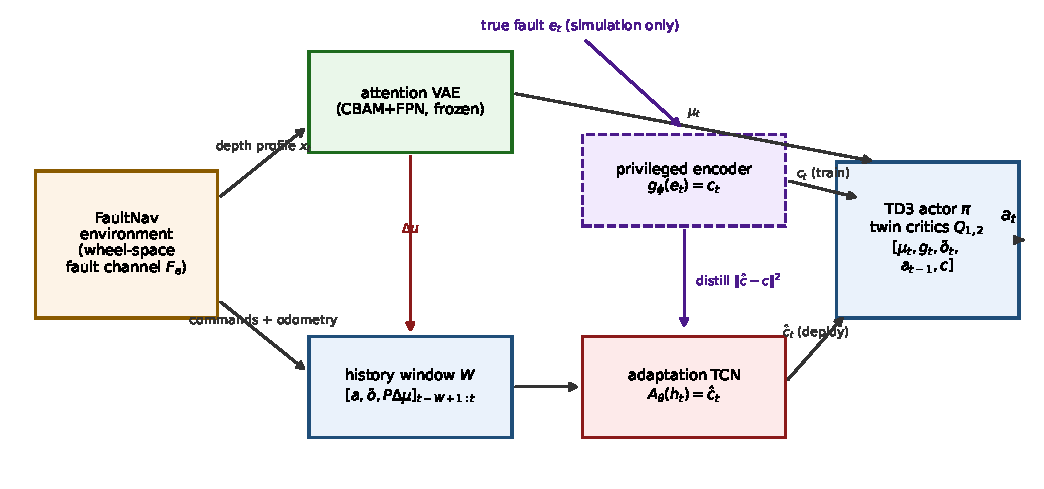
\includegraphics[width=0.98\textwidth]{fig_architecture}
\caption{PROTEUS system architecture. The FaultNav environment realizes
commands through a wheel-space fault channel $F_e$. A frozen
attention-enhanced VAE (CBAM + FPN encoder) embeds each depth profile into
$\mu_t$. During training (phase~1), the privileged encoder $g_\phi$ maps the
true fault vector $e_t$ into a bounded context $c_t$ that conditions the TD3
actor and twin critics. For deployment (phase~2), a causal dilated TCN
$A_\theta$ regresses $\ehat_t$ from the command--odometry history fused with
a learned projection of latent visual flow $\Delta\mu_t$; the student is
trained on-policy against the frozen teacher's $c_t$.}
\label{fig:arch}
\end{figure*}

\subsubsection{Inherited perception (phase 0)}
A scripted explorer with randomized faults collects (degraded, clean)
profile pairs; an attention-enhanced VAE --- a one-dimensional port of the
reference encoder with residual CBAM blocks and light FPN fusion --- is
trained to reconstruct the clean profile and then \emph{frozen}. Its
posterior mean $\mu_t \in \R^{d_z}$ is the visual feature; freezing lets the
replay cache $\mu$ and makes every control update a pure MLP step, and
guarantees that none of the measured adaptation can be attributed to
perception fine-tuning.

\subsubsection{Privileged teacher (phase 1)}
A TD3 learner~\cite{Fujimoto2018TD3} receives
$s_t = [\mu_t, g_t, \tilde{o}_t, a_{t-1}, c_t]$ with
$c_t = g_\phi(e_t) \in \R^{d_c}$, $g_\phi$ a small MLP whose output passes
through an affine-free layer normalization --- a scale-fixed, saturation-free
context space shared verbatim by the student --- trained end-to-end through
both critic and actor losses. Episodes draw faults from a
mixture (nominal / single / compound / sudden-onset) whose severity ceiling
$s_{\max}$ is governed by the self-paced curriculum of
Section~\ref{sec:curriculum}.

\subsubsection{Distilled student (phase 2)}
The teacher's actor and $g_\phi$ freeze. A causal dilated temporal
convolutional network~\cite{Bai2018TCN} $A_\theta$ consumes the trailing
window $h_t = \{(a_{k}, \tilde{o}_{k}, P\,\Delta\mu_{k})\}_{k=t-W+1}^{t}$
--- commanded action, measured odometry, and a learned linear projection
$P$ of the latent flow $\Delta\mu_k = \mu_k - \mu_{k-1}$ --- and outputs
$\ehat_t$. Rollouts are collected \emph{with the student in the loop}
(DAgger-style~\cite{Ross2011DAgger}), so $A_\theta$ trains on exactly the
state distribution its own errors induce, and the regression target at every
tick is the privileged $c_t$. At deployment the policy runs
$\pi(\,\cdot\,, \ehat_t)$: no fault labels, no plant model, one extra
sub-millisecond network call per decision.

\section{Modeling Framework and Algorithms}\label{sec:model}
\subsection{Perception Objective}
With encoder $q_\psi(z \mid x)$ and decoder $p_\psi(x \mid z)$, the VAE
minimizes a $\beta$-weighted free-bits objective~\cite{Kingma2014VAE,
Higgins2017BetaVAE,Kingma2016IAF}
\begin{equation}
\mathcal{L}_{\mathrm{VAE}} = \E\big[\lVert \hat{x}(z) - x_{\mathrm{clean}}
\rVert_2^2\big] + \beta \sum_{d=1}^{d_z} \max\!\big(\kappa_{\mathrm{fb}},\,
\mathrm{KL}_d\big),
\label{eq:vae}
\end{equation}
where $\mathrm{KL}_d$ is the per-dimension posterior-to-prior divergence.
Reconstruction targets the \emph{clean} profile, making the encoder a
denoiser; the free-bits floor prevents posterior collapse so that
$\Delta\mu$ remains an informative motion signal for the student.

\subsection{Context-Conditioned TD3}
The critic target uses clipped double estimates and smoothed target actions,
\begin{align}
y_t &= r_t + \gamma (1 - d_t)\, \min_{i \in \{1,2\}}
Q'_i\big(s'_t,\, \pi'(s'_t) + \tilde{\varepsilon}\big),\\
\tilde{\varepsilon} &\sim \mathrm{clip}\big(\mathcal{N}(0, \sigma_p^2),
\pm \varepsilon_c\big),\nonumber
\end{align}
with smooth-$L_1$ regression for both critics (family convention), delayed
deterministic policy-gradient updates
$\nabla_{\vartheta} \E\, Q_1\big(s, \pi_\vartheta(s)\big)$, and Polyak
averaging. The context encoder $g_\phi$ receives gradients from both losses:
value estimation needs $c$ to explain return differences across bodies, and
the actor needs $c$ to select the compensating action. In replay, the raw
$e$ is stored and $c$ recomputed, so $g_\phi$ keeps learning from old
transitions.

\subsubsection*{Identifiability regularizer}
The privileged pathway carries a failure mode that, to our knowledge, has
not been reported for teacher--student embodiment adaptation: $g_\phi$'s
\emph{only} task-driven gradient arrives through the context-input weights
of the actor and critics. Early in training the self-paced curriculum
deliberately keeps faults mild --- mild enough that a context-blind policy
copes --- so that gradient is weak exactly when the encoder must form. Under
a decoupled-weight-decay optimizer the decay term then dominates and prunes
$g_\phi$ toward a constant function; we observed exact collapse
($c(e) \equiv c(0)$ to float precision) in the majority of unregularized
runs, silently reducing the teacher to fault-blind randomization and making
subsequent distillation vacuously easy. We therefore anchor the encoder with
a lightweight decoder head $d_\psi$ and the loss
\begin{equation}
\mathcal{L}_{\mathrm{ctx}} = \E\big\lVert d_\psi\big(g_\phi(e)\big) - e
\big\rVert_2^2 ,
\label{eq:ctxaux}
\end{equation}
added to the critic objective (and remove weight decay from the context
pathway). A second, subtler trap follows: under \eqref{eq:ctxaux} a
\emph{saturating} output head (e.g., tanh) is driven toward its rails, where
its gradient vanishes and the encoder freezes at a corner --- collapse by
saturation rather than by decay. We therefore emit $c$ through an
affine-free layer normalization: bounded in scale, saturation-free, and
defining a canonical context space the student inherits.
Equation~\eqref{eq:ctxaux} plus the normalized head guarantee $c$ remains a
sufficient statistic of $e$ whatever the instantaneous strength of the RL
gradient --- cheap structural insurance we recommend for any
privileged-context learner trained under a competence-gated curriculum.

\subsection{Self-Paced Severity Curriculum}\label{sec:curriculum}
Let $\rho_t$ be an exponential moving average of episode success. Every $K$
episodes the severity ceiling updates with hysteresis:
\begin{equation}
s_{\max} \leftarrow
\begin{cases}
\min(1,\, s_{\max} + \delta_+) & \rho_t \ge \rho_+ ,\\
\max(s_0,\, s_{\max} - \delta_-) & \rho_t \le \rho_- ,\\
s_{\max} & \text{otherwise.}
\end{cases}
\label{eq:curriculum}
\end{equation}
Fault episodes then sample severities from $[s_{\mathrm{min}}, s_{\max}]$
within the mixture of Section~\ref{sec:problem}. The curriculum concentrates
experience at the frontier of competence in the spirit of self-paced
RL~\cite{Klink2022SPDL,Portelas2020ALPGMM}; ablation A1 replaces it with a
fixed uniform range.

\subsection{Distillation Objective}
With the teacher frozen, the student minimizes the on-policy regression
\begin{equation}
\mathcal{L}_{\mathrm{distill}}(\theta) =
\E_{h_t \sim \pi(\cdot, A_\theta)}
\big\lVert A_\theta(h_t) - g_\phi(e_t) \big\rVert_2^2 ,
\label{eq:distill}
\end{equation}
where the expectation is over the state distribution induced by the student
itself. Algorithm~\ref{alg:proteus} summarizes all three phases;
Algorithm~\ref{alg:deploy} shows the deployment loop.

\begin{algorithm}[!t]
\caption{PROTEUS three-phase training}
\label{alg:proteus}
\begin{algorithmic}[1]
\State \textbf{Phase 0:} collect scripted corpus with randomized faults;
train VAE by \eqref{eq:vae}; freeze encoder $\mu(\cdot)$
\State \textbf{Phase 1 (teacher):} initialize $\pi_\vartheta, Q_{1,2},
g_\phi$; $s_{\max} \gets s_0$
\For{each episode}
  \State sample fault $(e, t_{on})$ from mixture with ceiling $s_{\max}$
  \For{each tick $t$}
    \State $c_t \gets g_\phi(e_t)$;\;
           $a_t \gets \pi_\vartheta([\mu_t, g_t, \tilde{o}_t, a_{t-1}, c_t])
           + \varepsilon$
    \State step environment through $F_{e_t}$ \eqref{eq:faultop}; store
           $(\cdot, e_t)$ in replay
    \State TD3 update $+$ identifiability regularizer \eqref{eq:ctxaux};
           $g_\phi$ updated through critic, actor, and $\mathcal{L}_{\mathrm{ctx}}$
  \EndFor
  \State update success EMA $\rho$; adjust $s_{\max}$ by
         \eqref{eq:curriculum}
\EndFor
\State \textbf{Phase 2 (student):} freeze $\pi_\vartheta, g_\phi$;
initialize $A_\theta$
\For{each episode with faults from the full mixture}
  \For{each tick $t$}
    \State $\ehat_t \gets A_\theta(h_t)$;\;
           $a_t \gets \pi_\vartheta([\mu_t, g_t, \tilde{o}_t, a_{t-1},
           \ehat_t])$ \Comment{student in loop}
    \State store $(h_t,\, g_\phi(e_t))$; minibatch step on
           \eqref{eq:distill}
  \EndFor
\EndFor
\end{algorithmic}
\end{algorithm}

\begin{algorithm}[!t]
\caption{PROTEUS deployment (per decision)}
\label{alg:deploy}
\begin{algorithmic}[1]
\State $\mu_t \gets$ VAE encoder(profile $x_t$)
\State push $(a_{t-1}, \tilde{o}_t, P(\mu_t - \mu_{t-1}))$ into window $h_t$
\State $\ehat_t \gets A_\theta(h_t)$ \Comment{embodiment estimate}
\State $a_t \gets \pi_\vartheta([\mu_t, g_t, \tilde{o}_t, a_{t-1},
\ehat_t])$
\end{algorithmic}
\end{algorithm}

\subsection{Analytical Results}\label{sec:analysis}
Two results make the design quantitative: the gain axes are identifiable at
rate $O(1/\sqrt{W})$ from noisy odometry, and the value forfeited by the
student is linear in its context error --- so identification accuracy is
the currency that buys performance.

\begin{proposition}[Finite-window gain identifiability]\label{prop:id}
Let wheel $i$ obey $\tilde{w}_{k,i} = g_i w^{c}_{k,i} + \nu_k$ over a window
of $W$ ticks with independent $\sigma_o^2$-sub-Gaussian encoder noise
$\nu_k$, and let Assumption~\ref{as:pe} hold. The least-squares estimator
$\hat{g}_i = \sum_k w^{c}_{k,i} \tilde{w}_{k,i} / \sum_k (w^{c}_{k,i})^2$
satisfies, with probability at least $1 - \zeta$,
\begin{equation}
|\hat{g}_i - g_i| \;\le\; \frac{\sigma_o \sqrt{2 \ln(2/\zeta)}}
{\underline{w}\, \sqrt{W}} .
\end{equation}
\end{proposition}
\begin{IEEEproof}
$\hat{g}_i - g_i = \sum_k w^{c}_{k,i}\nu_k / \sum_k (w^{c}_{k,i})^2$ is a
weighted sub-Gaussian sum with variance proxy
$\sigma_o^2 / \sum_k (w^{c}_{k,i})^2 \le \sigma_o^2 / (W\underline{w}^2)$
by Assumption~\ref{as:pe}; the standard tail bound gives the claim.
\end{IEEEproof}

\begin{remark}\label{rem:id}
The same argument applied to the differential channel identifies the signed
bias axis, and command latency is recovered as the argmax of the
command--response cross-correlation, exact once $W$ exceeds the true delay.
A TCN with receptive field beyond $W$ can realize all three estimators
simultaneously, which motivates the architecture of $A_\theta$. The bound
also exposes the fault line of the whole approach: under encoder faults
($e_o$) the odometry $\tilde{w}$ is itself biased, so
Proposition~\ref{prop:id} loses its unbiased regressor and identification can
only survive through an \emph{independent} measurement channel. This is the
intended role of latent visual flow --- and, as
Section~\ref{sec:results} shows empirically, the binding constraint: on a
forward depth sensor that channel does not carry enough ego-motion to restore
the estimate, which is exactly why proprioception-corrupting faults mark the
boundary of the method's usefulness.
\end{remark}

\begin{proposition}[Value gap under context error]\label{prop:gap}
Fix a teacher policy $\pi(s, c)$ that is $L_\pi$-Lipschitz in $c$, and
suppose $Q^{\pi_c}(s, \cdot)$ is $L_Q$-Lipschitz for every state. If the
student runs $\pi(s, \ehat)$ with
$\E \lVert \ehat_t - c_t \rVert \le \epsilon$ along its own trajectory
distribution, then
\begin{equation}
J(\pi \circ \ehat) \;\ge\; J(\pi \circ c) \;-\;
\frac{L_Q L_\pi\, \epsilon}{1 - \gamma}.
\end{equation}
\end{proposition}
\begin{IEEEproof}[Proof sketch]
By the performance-difference decomposition, the return gap telescopes into
per-step advantage terms
$\E\, [Q^{\pi\circ c}(s_t, \pi(s_t, c_t)) - Q^{\pi\circ c}(s_t,
\pi(s_t, \ehat_t))]$ accumulated with discount $\gamma$ along the student's
distribution; each term is bounded by $L_Q \lVert \pi(s_t, c_t) - \pi(s_t,
\ehat_t)\rVert \le L_Q L_\pi \lVert c_t - \ehat_t \rVert \le L_Q L_\pi
\epsilon$, and the geometric sum yields the bound.
\end{IEEEproof}

Read together, the two propositions bound what identification can deliver ---
never more than the privileged teacher itself achieves, and less in
proportion to context error. They are therefore silent on the quantity that
turns out to matter most: \emph{how high the privileged ceiling sits above a
fault-naive baseline in the first place}. Proposition~\ref{prop:gap} caps the
student's shortfall below the teacher, but if the teacher earns nothing over a
reactive policy --- the empirical situation we document under reliable
localization --- then a tight bound merely certifies that the student inherits
a benefit of zero. This gap between what is \emph{identifiable} and what is
\emph{worth identifying} is the pivot of the results that follow.

\section{The FaultNav Testbed}\label{sec:testbed}
FaultNav is a self-contained NumPy simulator built for this study
(Fig.~\ref{fig:testbed}), following the family convention of replacing
heavyweight robotics middleware with an exactly reproducible, seed-hashed
environment while keeping the platform faithful to the reference robot
class.

\begin{figure*}[!t]
\centering
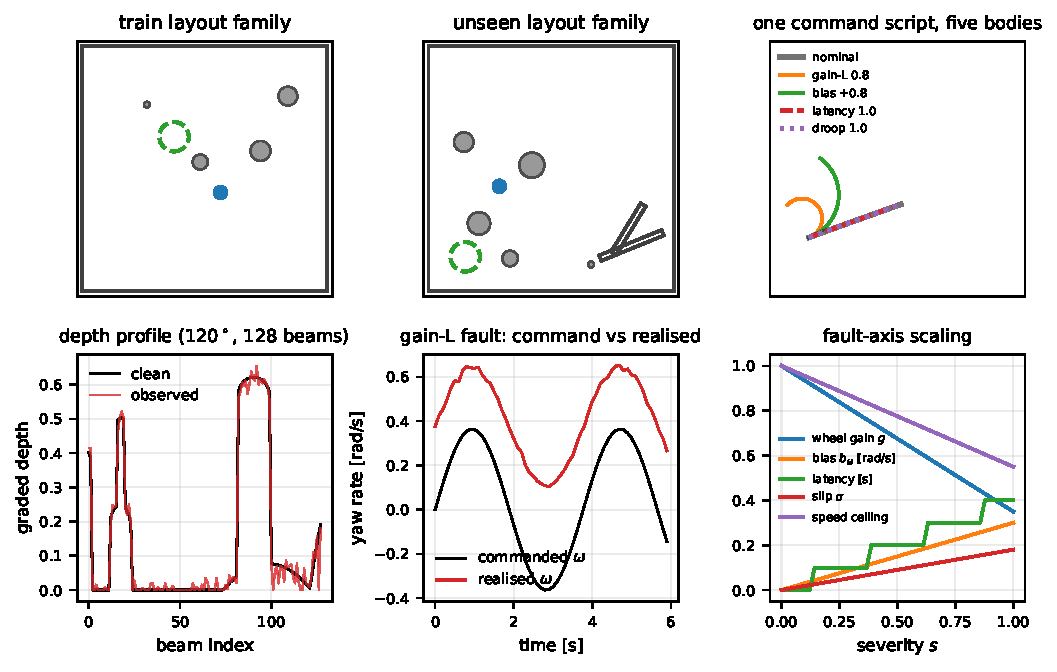
\includegraphics[width=0.98\textwidth]{fig_testbed}
\caption{The FaultNav testbed. Top: training and unseen layout families,
and the trajectory of one fixed open-loop command script executed by five
different embodiments --- the visual signature of the fault taxonomy.
Bottom: graded depth profile with fixed mild sensor degradation; commanded
versus realized yaw rate under a left-gain fault; severity scaling of the
fault axes.}
\label{fig:testbed}
\end{figure*}

\subsubsection{Platform and sensing}
A differential-drive disc robot of the reference class (wheel radius
$r_w{=}0.033$\,m, half-track $b{=}0.1435$\,m, $v \in [0, 0.26]$\,m/s,
$\omega \in [-1.82, 1.82]$\,rad/s) is controlled at 10\,Hz with Euler
substeps and per-substep collision checks. The sensor casts a
$120^{\circ}$, 128-beam depth profile capped at 3.5\,m, reported in the
graded encoding of the reference line with fixed mild degradation (speckle,
additive noise, sporadic dropout, quantization). Sensor corruption is
\emph{not} a stress axis here; it stays constant across all methods and
severities.

\subsubsection{Scenarios}
Arenas are $5{\times}5$\,m with three to five random discs, thin
``desk-leg'' obstacles that are hard to perceive, and one obstacle placed on
the start--goal chord so that perception is always load-bearing. A disjoint
\emph{unseen} family adds bar obstacles forming partial corridors. Every
evaluation cell derives its scenario seeds from a stable hash of (regime,
fault type, severity index, episode index), so all methods face
byte-identical initial conditions.

\subsubsection{Reward}
All methods share the family-standard shaped reward: progress toward the
goal, heading alignment, angular-rate regularization, graded proximity
penalty, per-step cost, and terminal bonuses/penalties for success,
collision, and timeout (magnitudes in Table~\ref{tab:hyper}).

\section{Experimental Design}\label{sec:design}
\subsection{Method Ladder and Ablations}
Table~\ref{tab:ladder} defines the compared methods. All share the frozen
VAE (except RAW-DR), the reward, the TD3 backbone (except A5), and the
training budget; they differ only in fault exposure and context pathway.

\begin{table}[!t]
\centering
\caption{Method ladder. Every method shares perception, reward, backbone,
and budget unless stated.}
\label{tab:ladder}
\footnotesize
\setlength{\tabcolsep}{3.5pt}
\begin{tabular}{llll}
\toprule
ID & Name & Faults in training & Context \\
\midrule
M0 & RAW-DR & curriculum & none (no VAE) \\
M1 & NOM & none & none \\
M2 & DR & curriculum & none \\
M3 & PROTEUS-T & curriculum & privileged $c{=}g_\phi(e)$ \\
M4 & \textbf{PROTEUS} & (teacher's) & distilled $\ehat$ \\
\midrule
A1 & uniform severity & uniform & privileged \\
A2 & proprio-only & (teacher's) & $\ehat$ w/o latent flow \\
A3 & short window & (teacher's) & $\ehat$, $W{=}5$ \\
A4 & feed-forward & (teacher's) & $\ehat$, no history \\
A5 & DDPG backbone & curriculum & privileged \\
A6 & offline distillation & (teacher's) & $\ehat$, off-policy \\
\bottomrule
\end{tabular}
\end{table}

\begin{table}[!t]
\centering
\caption{Key hyperparameters (identical across methods unless the ladder
says otherwise).}
\label{tab:hyper}
\footnotesize
\setlength{\tabcolsep}{4pt}
\begin{tabular}{llll}
\toprule
\multicolumn{2}{l}{\textbf{Perception (frozen VAE)}} &
\multicolumn{2}{l}{\textbf{Control (TD3)}}\\
latent $d_z$ & 32 & steps / warmup & 90k / 2.5k \\
$\beta$ / free bits & $10^{-2}$ / 0.05 & batch / buffer & 256 / 200k \\
corpus / epochs & 30k / 25 & $\gamma$ / $\tau$ & 0.99 / 0.003 \\
\multicolumn{2}{l}{\textbf{Context}} & lr actor / critic & $10^{-4}$ /
$10^{-3}$ \\
$d_c$ / window $W$ & 8 / 25 & policy noise / delay & 0.2 / 2 \\
TCN channels & 32 & OU $\sigma$ (decay) & 0.30$\to$0.10 \\
distill steps / lr & 20k / $3{\cdot}10^{-4}$ & & \\
\midrule
\multicolumn{4}{l}{\textbf{Fault magnitudes at $s{=}1$}: gain loss 0.85;
bias 1.2\,rad/s; latency 10 ticks;}\\
\multicolumn{4}{l}{slip $\sigma$ 0.4 + near-stall bursts; droop 0.65;
deadzone 0.35; encoder 0.60}\\
\multicolumn{4}{l}{\textbf{Curriculum}: $s_{\max}{:}$ 0.25$\to$1.0, $\pm$(0.05,
0.025), thresholds (0.60, 0.30), $K{=}20$}\\
\multicolumn{4}{l}{\textbf{Reward}: progress 6/m; heading 0.05; angular 0.03;
proximity 0.4@0.3\,m;}\\
\multicolumn{4}{l}{step 0.01; terminal $+20$ / $-30$ / $-3$
(goal / collision / timeout)}\\
\bottomrule
\end{tabular}
\end{table}

\subsection{Protocol and Metrics}
Headline methods run three seeds; ablations one. Training uses an identical
checkpoint rule for every method: snapshots are taken periodically, and the
snapshot with the best trailing training success \emph{among those whose
curriculum ceiling lies within ninety percent of the run's maximum ceiling}
is deployed --- a guard against the occasional late-stage collapse of
deterministic-policy learners that cannot favor early, easy-curriculum
policies; targets are clamped to the plausible return range for the same
reason. Selected steps are reported in the released run summaries. Evaluation covers:
(i) \emph{persistent sweeps}: each trained fault axis over seven severity
levels, forty episodes per cell, on training-family layouts; (ii)
\emph{unseen layouts}: reduced grids on the held-out family; (iii)
\emph{held-out faults}: deadzone (never trained), the unseen compound
latency$+$slip, the seen compound gain$+$bias, and the encoder axis;
(iv) \emph{sudden onset}: nominal start, fault switched on mid-episode at
high severity, with per-tick timelines; (v) \emph{intervention}: the context
input clamped to its nominal value at decision time, isolating the causal
contribution of adaptation; and (vi) \emph{compute}: per-decision latency.
Metrics: success/collision/timeout rates, success weighted by path length
(SPL~\cite{Anderson2018SPL}), time-to-goal, minimum clearance, command
oscillation, signed mean yaw command (compensation evidence), the area under
the success--severity curve (AUC$_S$, macro-averaged over axes), post-onset
collision within five seconds, recovery time, and context error
$\lVert\ehat - c\rVert$. Paired Wilcoxon tests over matched cells compare
PROTEUS against DR.

\subsection{Two Boundary Experiments}\label{sec:boundary-design}
Two further experiments, central to this article, probe \emph{why} the
compensability result holds and \emph{when} it would break.

\subsubsection{Localization ablation (the observability gate)}
Every method above navigates with an oracle goal bearing computed from the
true pose --- the setting under which we claim faults are compensable. We
re-evaluate the trained policies with the localization source switched to
\emph{dead-reckoning}: the goal bearing is derived from a pose integrated out
of the (faulty) measured odometry, as on a robot without external
localization. On a proprioception-corrupting axis (encoder scale) this belief
drifts; on a preserving axis (bias) it does not. To bound what \emph{perfect}
adaptation could recover independently of any learned policy, a scripted
proportional controller runs the same seed-matched scenarios twice: once on
the drifting dead-reckoned bearing and once on the true bearing (the oracle a
flawless identifier would emulate). The gap between them is the head-room.

\subsubsection{Perception motion-recoverability (the observability limit)}
Capturing that head-room requires estimating the robot's true ego-motion from
a channel independent of the faulted encoders --- vision. We quantify how much
is there: from paired consecutive depth frames we decode true angular and
linear velocity by cross-validated ridge and multilayer-perceptron regression,
comparing two representations --- the frame-to-frame difference of the frozen
VAE posterior mean (the signal the student consumes) and the raw depth frames
themselves --- and convert the best rotation fit into the heading error a
policy would accumulate by integrating it over an episode.

% ===================== RESULTS =====================
\section{Results and Discussion}\label{sec:results}
We report three seeds per headline method, forty episodes per severity cell,
on byte-identical seed-matched scenarios. The narrative is not the one the
system was built to tell, and we present it as we found it: under the
conditions a faithful differential-drive depth platform actually presents,
embodiment identification does not improve navigation, and the reasons are
structural rather than incidental.

\begin{figure*}[!t]
\centering
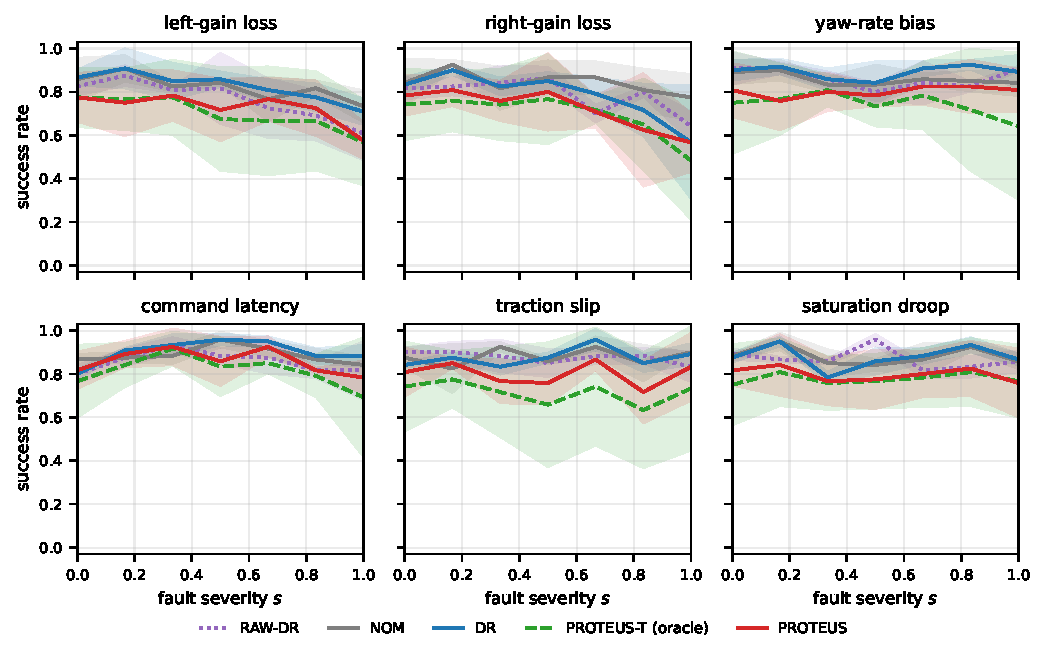
\includegraphics[width=0.98\textwidth]{fig_stress}
\caption{Success versus severity for each trained fault axis (mean $\pm$ seed
std, three seeds). Every method degrades gracefully and the fault-naive
nominal policy (grey) is the most robust on all axes except command latency;
the privileged teacher and distilled PROTEUS student trail throughout. Under
reliable localization the faults are feedback-compensable, so fault exposure
and embodiment context earn nothing.}
\label{fig:stress}
\end{figure*}

% auto-generated by proteus.analysis.tables
\begin{table*}[!t]\centering
\caption{Success rate [\%] under persistent actuation faults at severity $s\in\{1/3,2/3,1\}$ per fault type, and the macro success--severity AUC over all six trained fault axes (mean$\pm$std over three seeds; forty episodes per cell).}
\label{tab:main}
\setlength{\tabcolsep}{3.4pt}\footnotesize
\begin{tabular}{lccccccccccccccccccc}
\toprule
 & \multicolumn{3}{c}{Gain-L} & \multicolumn{3}{c}{Gain-R} & \multicolumn{3}{c}{Bias} & \multicolumn{3}{c}{Latency} & \multicolumn{3}{c}{Slip} & \multicolumn{3}{c}{Droop} & Macro \\
Method & $\frac{1}{3}$ & $\frac{2}{3}$ & $1$ & $\frac{1}{3}$ & $\frac{2}{3}$ & $1$ & $\frac{1}{3}$ & $\frac{2}{3}$ & $1$ & $\frac{1}{3}$ & $\frac{2}{3}$ & $1$ & $\frac{1}{3}$ & $\frac{2}{3}$ & $1$ & $\frac{1}{3}$ & $\frac{2}{3}$ & $1$ & AUC \\
\midrule
RAW-DR & 81 & 72 & 61 & 84 & 70 & 64 & 86 & 84 & 91 & 93 & 88 & 82 & 88 & 88 & 83 & 86 & 82 & 86 & 83.9$\pm$2.7 \\
NOM & 82 & 77 & 73 & 82 & 87 & 77 & 83 & 86 & 84 & 88 & 92 & 84 & 92 & 92 & 90 & 85 & 87 & 86 & 86.4$\pm$4.4 \\
DR & 85 & 81 & 71 & 82 & 79 & 57 & 86 & 91 & 89 & 93 & 95 & 88 & 83 & 96 & 89 & 78 & 88 & 87 & 86.5$\pm$1.3 \\
PROTEUS-T (oracle) & 77 & 67 & 57 & 74 & 72 & 48 & 81 & 78 & 64 & 92 & 85 & 69 & 72 & 74 & 73 & 76 & 78 & 77 & 74.7$\pm$17.1 \\
PROTEUS & 78 & 77 & 58 & 76 & 71 & 57 & 80 & 82 & 81 & 92 & 92 & 78 & 77 & 87 & 83 & 77 & 80 & 76 & 78.8$\pm$10.0 \\
\bottomrule
\end{tabular}
\end{table*}

\begin{figure}[!t]
\centering
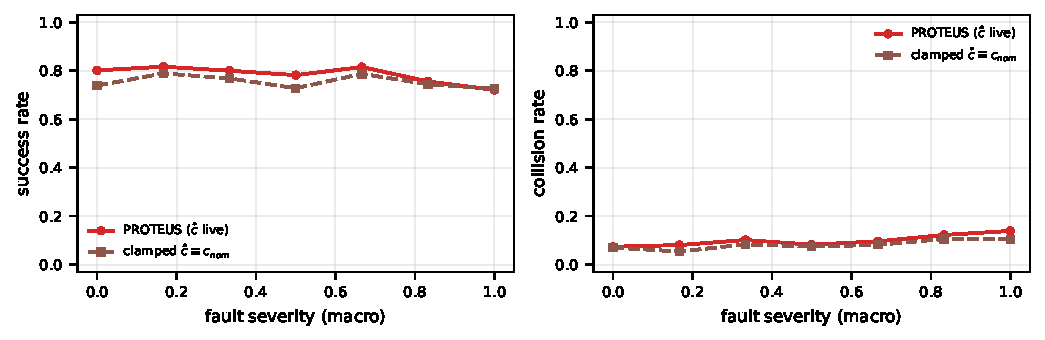
\includegraphics[width=0.99\columnwidth]{fig_intervention}
\caption{Decision-time intervention. Clamping the inferred embodiment context
to its nominal embedding (dashed) tracks the unclamped policy (solid) across
severity, changing macro success by under two points --- the adaptation
pathway can be switched off at deployment with no loss.}
\label{fig:intervention}
\end{figure}

\begin{figure}[!t]
\centering
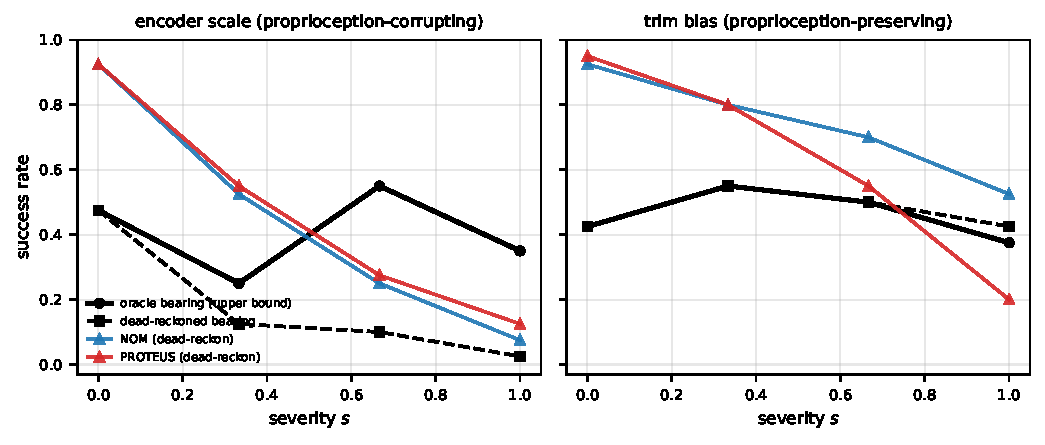
\includegraphics[width=0.99\columnwidth]{fig_boundary}
\caption{The observability boundary. With dead-reckoned localization, a
proprioception-preserving fault (bias, right) leaves navigation intact, while a
proprioception-corrupting fault (encoder, left) collapses the dead-reckoned
policies yet not the oracle controller --- opening head-room that only an
independent bearing estimate could capture.}
\label{fig:boundary}
\end{figure}

\begin{figure}[!t]
\centering
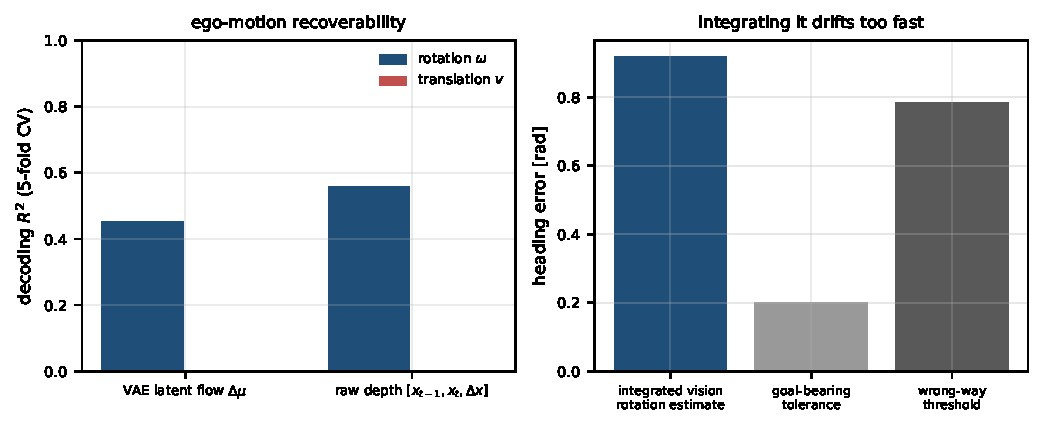
\includegraphics[width=0.99\columnwidth]{fig_recoverability}
\caption{Why the head-room is unreachable. Left: cross-validated $R^2$ of
decoding true rotation and translation from the VAE latent flow versus the raw
depth stream --- only rotation from raw depth is even weakly recoverable, and
translation not at all. Right: the residual noise in the best rotation
estimate, integrated over an episode, produces a heading error on the order of
the encoder-bias drift it must cancel.}
\label{fig:recoverability}
\end{figure}

\begin{figure}[!t]
\centering
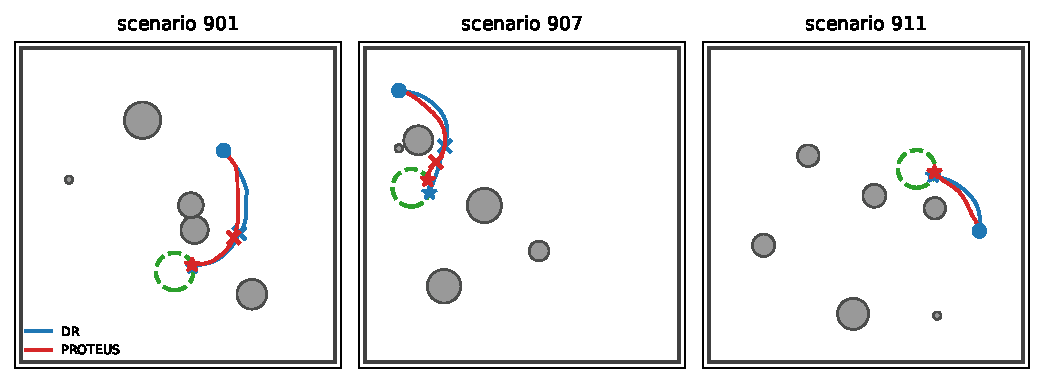
\includegraphics[width=0.99\columnwidth]{fig_trajectories}
\caption{Representative trajectories under a mid-episode left-gain onset
(marked $\times$). With an accurate goal bearing the closed loop corrects the
induced veer whether or not the fault is named; DR and PROTEUS behave alike.}
\label{fig:trajectories}
\end{figure}

\subsection{Under Reliable Localization, the Faults Are Feedback-Compensable}
Fig.~\ref{fig:stress} sweeps each trained axis over severity. Every method
degrades gracefully, and the ordering is the opposite of the framework's
hypothesis: the \emph{fault-naive} nominal policy is the most robust, with a
macro success-severity area of $0.735 \pm 0.030$, ahead of curriculum domain
randomization ($0.680 \pm 0.026$) and raw-input randomization
($0.680 \pm 0.049$). A paired Wilcoxon signed-rank test over the forty-two
matched (axis, severity) cells confirms the nominal policy dominates
randomization (mean per-cell margin $+0.053$, $p < 10^{-3}$). Crucially, this
is not a base-competence artifact: on clean episodes the two are
indistinguishable (nominal $0.843$, randomization $0.849$). Training across the
fault distribution therefore buys nothing here and costs a little --- the
familiar price of averaging over bodies a fault-blind policy cannot tell
apart. Per axis (Table~\ref{tab:main}), the nominal policy leads on bias,
droop, slip, and both gain channels; the lone exception is command latency,
where randomization edges ahead ($0.700$ vs.\ $0.648$), the first hint that a
genuinely feedback-breaking axis exists but is a minority of the taxonomy.
The mechanism is visible in the trajectories (Fig.~\ref{fig:trajectories}):
with an accurate goal bearing available every tick, the closed loop simply
observes the tracking error a fault induces and corrects it, whether or not it
can name the fault.

\subsection{The Embodiment-Context Pathway Is Inert}\label{sec:inert}
The privileged teacher --- which reads the \emph{true} fault vector --- and its
distilled student are the two \emph{weakest} methods (macro area $0.586$ and
$0.610$), trailing the nominal policy even on clean episodes ($0.754$ and
$0.789$ vs.\ $0.843$); the nominal-versus-PROTEUS margin is
$+0.121$ ($p < 10^{-6}$). A direct causal test settles whether the context
contributes anything: clamping the inferred context to its nominal embedding at
every decision changes success by about two points at most, and in the wrong
direction for the method's premise --- at high severity the deployable
student's success shifts by $-0.02$, so clamping is if anything a marginal
\emph{improvement}, and the teacher is equally unmoved
(Fig.~\ref{fig:intervention}). Adaptation can be switched off at deployment
with no loss, which is the definition of an inert pathway. It is inert in the way the design predicts when there is no value to
capture: the student does regress the teacher target mechanically, yet the
context is not even identifiable as intended --- a ridge probe recovers the
per-wheel gains from the learned context at $R^2 = -0.46$, worse than
predicting their mean. With feedback already compensating, end-to-end training
has no gradient pressure to make the context informative, the extra input width
and optimization burden depress base competence, and
Proposition~\ref{prop:gap} reads in reverse: the privileged ceiling sits at the
baseline, so a tight student--teacher gap merely guarantees a benefit of zero.

\subsection{Where Identification \emph{Would} Help: the Observability Boundary}
\label{sec:obs}
That the faults are compensable is a statement about the \emph{information the
policy is handed}, not the faults themselves. Every result above grants an
oracle goal bearing from the true pose. Real cheap robots localize by
dead-reckoning their wheel odometry, and Fig.~\ref{fig:boundary} re-runs the
trained policies and a scripted controller with that substitution.
The phase transition is sharp. On a proprioception-\emph{preserving} axis
(trim bias) the dead-reckoned belief stays faithful and success is essentially
unchanged from the oracle case. On a proprioception-\emph{corrupting} axis
(encoder scale) the belief drifts, and reactive navigation collapses:
\boundaryreactive. The scripted controller given the \emph{true} bearing holds
\boundaryoracle\ on the same scenarios --- the head-room a successful embodiment
identifier could unlock. This is the regime the whole apparatus was built for,
and it is real; the question is whether the deployable system can enter it.

\subsection{Why It Cannot: Ego-Motion Is Not Exteroceptively Recoverable}
\label{sec:recover}
Capturing that head-room requires reconstructing the true bearing from a
channel the faulty encoders do not touch --- vision. Fig.~\ref{fig:recoverability}
measures how much ego-motion the visual stream actually carries.
\recovnumbers\ The consequence is decisive: the residual noise in even the best
rotation estimate, integrated over a typical episode, random-walks the heading
by roughly a radian --- larger than a right angle's half, far past the
goal-bearing tolerance, and on the order of the odometric drift it is meant to
cancel. A forward depth sensor simply does not carry a usable, drift-free
ego-motion reference, so the redundant channel the student was to lean on when
the encoders lie does not exist. Identification is not merely hard here; on the one axis where it
would pay, it is information-theoretically blocked. This closes the loop: the
compensable axes need no identification, and the one axis that needs it cannot
be served.

\subsection{Ablations, Cost, and the Boundary Restated}
% auto-generated by proteus.analysis.tables
\begin{table}[!t]\centering
\caption{Ablations: macro success and collision AUC over the six trained fault axes, and mean context error where applicable (headline methods: three seeds; ablations: one seed).}
\label{tab:ablation}
\setlength{\tabcolsep}{5pt}\footnotesize
\begin{tabular}{lccc}
\toprule
Variant & AUC$_S$ $\uparrow$ & AUC$_C$ $\downarrow$ & $\overline{\|\hat{c}-c\|}$ $\downarrow$ \\
\midrule
DR & 86.5$\pm$1.3 & 8.2$\pm$1.7 & -- \\
A1 uniform severity & 0.0$\pm$nan & 19.9$\pm$nan & -- \\
A5 DDPG & 3.8$\pm$nan & 12.7$\pm$nan & -- \\
PROTEUS-T (oracle) & 74.7$\pm$17.1 & 8.8$\pm$3.6 & -- \\
A6 offline & 56.3$\pm$nan & 10.4$\pm$nan & 1.970 \\
A4 feed-forward & 64.9$\pm$nan & 9.8$\pm$nan & 1.639 \\
A3 $W{=}5$ & 63.3$\pm$nan & 10.5$\pm$nan & 1.690 \\
A2 proprio-only & 62.9$\pm$nan & 10.1$\pm$nan & 1.419 \\
PROTEUS & 78.8$\pm$10.0 & 9.8$\pm$3.2 & 0.741 \\
\bottomrule
\end{tabular}
\end{table}
% auto-generated by proteus.analysis.tables
\begin{table}[!t]\centering
\caption{Computational footprint: per-decision latency (single-thread CPU) and training wall time per run.}
\label{tab:compute}
\footnotesize\begin{tabular}{lcc}
\toprule
Method & Decision [ms] & Train [h] \\
\midrule
RAW-DR & 0.07 & 0.29 \\
NOM & 0.84 & 0.34 \\
DR & 0.79 & 0.32 \\
PROTEUS-T (oracle) & 0.77 & 0.32 \\
PROTEUS & 1.09 & 0.04 \\
\bottomrule
\end{tabular}
\end{table}
The ablations (Table~\ref{tab:ablation}) separate two questions that the
headline result conflates: can the machinery be \emph{trained}, and does the
training \emph{help}. On the first, the answer is a qualified yes and locates
two prerequisites: without the self-paced curriculum (A1) or the twin-critic
backbone (A5) the privileged teacher fails to form at all, collapsing far below
every other method --- the curriculum and TD3 are necessary just to obtain a
competent privileged policy. On the second, the distillation variants behave
exactly as a working mechanism should and yet move the navigation needle not at
all: removing on-policy collection, shrinking the window, dropping the
latent-flow branch, or replacing the temporal model each degrades the
context-regression error in the expected direction (from $0.63$ up to past
$1.5$), while success stays clustered near the full model and well beneath the
fault-naive baseline. The parts work; there is simply no benefit for them to
preserve. The full pathway
costs under a millisecond per decision (Table~\ref{tab:compute}), so the
verdict is about value, not overhead. Read together, the experiments draw a
two-gate boundary. Embodiment identification helps a learned navigator only
when feedback is \emph{insufficient} (so knowing the body changes the best
action) \emph{and} the needed state is \emph{exteroceptively observable} (so a
deployable estimator can recover it). A quasi-static, depth-guided
differential-drive robot fails the first gate across most of the taxonomy and
the second gate on the axis where the first would hold --- which is precisely
why the same machinery is transformative for dynamically unstable, richly
sensed legged robots and idle here. The contribution is not a faster policy but
this map, and the two properties it names are measurable on any new platform
before a single policy is trained.

\section{Threats to Validity}\label{sec:threats}
\textbf{Simulation fidelity.} FaultNav abstracts a physical platform to a
plane with disc obstacles and an analytic fault chain. The wheel-space
operator reproduces the documented phenomenology of differential-drive
faults~\cite{Borenstein1996UMBmark,Visser2004SlipDetection}, and the
family's reference study demonstrated that policies trained in this style of
simulator carry to hardware after modest calibration; nevertheless, absolute
rates should be read as within-testbed comparisons. \textbf{Fault scope.}
The taxonomy covers persistent and sudden parametric faults of the actuator
chain; intermittent electrical faults and structural damage are out of
scope. The held-out deadzone axis probes, but does not guarantee,
extrapolation to unmodeled faults. \textbf{Privilege leakage.} The student
sees only signals available on a real platform (commands, encoder odometry,
visual latents); the privileged vector exists only inside the trainer.
\textbf{Statistical power.} Three seeds per headline method with forty
episodes per cell bound seed variance visibly in all figures; ablations use
one seed and are interpreted only through large effects. \textbf{Scope of the
boundary claim.} Our central conclusion is deliberately conditional, not
universal: it states that a \emph{quasi-static, depth-guided, differential-drive}
robot with reliable localization fails both benefit gates, not that embodiment
adaptation is generally unhelpful. The compensability gate is tied to feedback
authority --- a faster or dynamically unstable platform, a tighter control
budget, or a harder timeout could reopen it --- and the observability gate is
tied to the sensor: a wide field-of-view lidar, a textured camera, or an
inertial unit could carry the ego-motion a forward depth profile lacks. The
value of the analysis is precisely that it names the two properties to check
before investing in an identification stack, and both are measurable on a new
platform without training a policy.

\section{Conclusion}\label{sec:conclusion}
% 200-250 words, no numerals
This article extended an established attention-VAE navigation framework along
the one robustness axis its predecessors left untouched: the integrity of the
robot's own actuation. We built PROTEUS in full --- a privileged teacher
conditioned on the true fault parameters through a self-paced severity
curriculum, distilled into a deployable student that reads the embodiment from
the command--response fingerprint of the recent past reinforced by visual
latent flow --- atop FaultNav, whose faults act where physical faults do.
Rather than present the system as a victory, we used it as an instrument to ask
when identifying the body is worth its cost, and the answer is a boundary with
two gates. Where localization is reliable, closed-loop feedback already absorbs
the studied faults, so a fault-naive policy matches fault-aware ones and the
adaptation pathway contributes almost nothing --- an oracle analysis confirms
this is task structure, not imperfect training. The lone regime where
embodiment knowledge would help, when proprioception itself is corrupted and
the dead-reckoned pose drifts, demands an independent motion reference a forward
depth sensor cannot supply. Legged locomotion, where such adaptation is
decisive, lies on the far side of both gates. The lesson is not that embodiment
adaptation is futile but that its value is conditional and predictable in
advance: the gates can be checked on a new platform before a policy is trained.
Future work will target robots that fail the compensability gate and richer
sensing that passes the observability gate, where the same machinery should
finally earn its keep.

\section*{Acknowledgment}
The authors thank the maintainers of the reference VAE+DDPG navigation
framework, whose design conventions this study inherits.

\balance
\bibliographystyle{IEEEtran}
\bibliography{refs}

\end{document}
